\section{Opportunistisches Vorgehen und seine Folgen}

\textbf{Opportunistisches Vorgehen} (s. Abbildung~\ref{fig:opportunistischeentwicklung}) entspricht eher einem \textit{Trial \& Error} bei der Entwicklung von Software:

\begin{enumerate}
    \item es wird über die Anforderungen des Programms nachgedacht
    \item die Anforderungen werden implementiert
    \item es wird zwischendurch immer wieder durch den Entwickler getestet, ob die Software funktioniert und den Anforderungen entspricht
\end{enumerate}


\begin{figure}
    \centering
    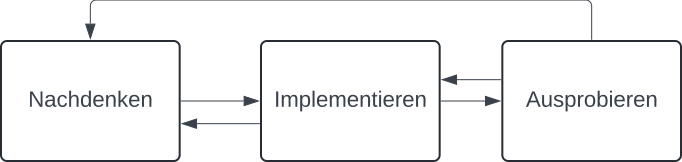
\includegraphics[scale=0.4]{chapters/Uebersicht ueber die Phasen des Entwicklungszyklus/img/opportunistischeentwicklung}
    \caption{Vorgehen bei \textit{opportunistischer} Softwareentwicklung. ``Testing`` entspricht hier einem bloßen ``Ausprobieren`` der umgesetzten Anforderungen. (Quelle: in Anlehnung an \cite[14, Abb. 2.1]{Wed09})}
    \label{fig:opportunistischeentwicklung}
\end{figure}

\noindent
Zwischen den einzelnen Phasen wird immer wieder hin- und hergesprungen, mit folgenden Konsequenzen:


\begin{itemize}
    \item \textbf{zu langsamer Fortschritt}: Man hält sich an kleineren Dingen auf und versucht diese zu perfektionieren.
    Eine genaue Anforderungsanalyse bzw. ein ``Plan``, der sich an den Mindestanforderungen orientiert und nach dem man entwickelt, hätte dies verhindern können.
    \item \textbf{schlechte Qualität}: Durch das ewige Herumprobieren und Nachbessern kommt man in Zeitverzug und einigt sich am Ende auf eine Lösung, die eher schlechtem Design entspricht
    \item  \textbf{Anforderungen übersehen / falsch verstanden}: Erneute Anpassungen notwendig, weil der Auftraggeber unzufrieden mit dem Ergebnis ist
    \item \textbf{kritische Fehler übersehen}: (systematisches) \textit{Ausprobieren} ersetzt kein \textit{automatisiertes Testing}, Änderungen können Fehler verursachen, die man beim manuellen Testing nicht berücksichtigt (\textit{Edge-cases})
    \item \textbf{schwierige Teamarbeit}: Absprache mit anderen im Team schwierig (\textit{planen}), wenn keine Anforderungen existieren bzw. die erst im Laufe der Zeit klar werden.
\end{itemize}

\noindent
Dieses Vorgehen hat auch Auswirkungen auf die Qualität des Quellcodes und der Architektur der Software. \textit{Martin} benennt hierfür folgende Symptome (vgl.~\cite[85]{Mar03}):

\begin{tcolorbox}[title=Symptoms of Poor Design]
    \begin{enumerate}
        \item \textbf{Rigidity} - The design is hard to change.
        \item \textbf{Fragility} - The design is easy to break.
        \item \textbf{Immobility} - The design is hard to reuse.
        \item \textbf{Viscosity} - It is hard to do the right thing.
        \item \textbf{Needless Complexity} - Overdesign.
        \item \textbf{Needless Repetition} - Mouse abuse.
        \item \textbf{Opacity} - Disorganized expression.
    \end{enumerate}
\end{tcolorbox}

